\documentclass[10pt, conference, compsocconf]{IEEEtran}

\usepackage[bookmarks=true]{hyperref}
\usepackage{epsfig}
\usepackage{amsmath,amssymb,amsfonts,latexsym}
\usepackage{enumerate}
\usepackage{xspace}
\usepackage{epsf,picinpar}
\usepackage{varioref}
\usepackage{colortbl,multirow,hhline}
\usepackage{listings}
\usepackage{amssymb}
\usepackage{colortbl,multirow,hhline}
\usepackage{algorithmic}
\usepackage{algorithm}
\usepackage{caption}
\usepackage[normalem]{ulem}
\usepackage{xcolor}
\usepackage{pifont}
\usepackage{xcolor,colortbl}
\usepackage{url}
\usepackage{balance}
\usepackage{graphicx, subfigure}
\usepackage{longtable}
\usepackage{lscape}
\usepackage{multirow}
\usepackage{listings}
\usepackage{framed}
\usepackage{morefloats}
\usepackage[T1]{fontenc}
\usepackage{array}
\usepackage{pdfpages}
\usepackage{fancybox}
\usepackage{amsmath}
\usepackage{flushend}
\usepackage{booktabs}
\usepackage{enumitem}
\usepackage{pbox}
\usepackage[bottom]{footmisc}

\renewcommand{\ttdefault}{cmr}

\newcommand{\source}[1]{\caption*{Source: {#1}}}
\newcommand{\limit}[1]{\textcolor{red}{\ding{46}~Page limit:~#1}\\}
\newcommand{\todo}[1]{\textcolor{blue}{\ding{46}~#1}} 
\newcommand{\ie}{\emph{i.e.,}\xspace}
\newcommand{\eg}{\emph{e.g.,}\xspace}
\newcommand{\etc}{etc.\xspace}
\newcommand{\etal}{\emph{et~al.}\xspace} 
    
\begin{document}

\title{
	\todo{Title}
}

\author{
	\IEEEauthorblockN{Sander Ronde}
	\IEEEauthorblockA{s.j.p.m.ronde@student.vu.nl\\
		Student number: 2639938\\
		Supervisor: Ivano Malavolta\\
		\\
		\today
	}
}

\maketitle

\begin{abstract}
	Since 2018, a set of technologies together referred to as Web Components are supported in all major browsers. Web Components are a set of technologies that enable support for the creation of custom HTML elements, thereby allowing for encapsulation of functionally and semantically related code. In this respect, they are similar to JavaScript (JS) frameworks, with the exception that these created elements (also called Web Components) have no dependencies and do not require any additional code to function. As such, any component such as a button, checkbox, or switch written using Web Components functions regardless of the JS framework used on a given page. This contrasts with code written using a JS framework, which generally requires that framework to be loaded on the page.

There are various reasons for developers to migrate an existing set of components (generally referred to as a component library) from a JS framework to Web Components. In this paper, we present a case study performed at the software company 30MHz, tackling such a scenario for one of these JS frameworks, namely the migrating of a set of Angular components to Web Components. Angular is one of the more popular JS frameworks for building web applications. It also suffers from the previously mentioned issue of components written in Angular not being usable in other JS frameworks. The migration to Web Components presents a solution to this issue.

In evaluating the quality and performance of the resulting Web Components, we find the load time of the JS code to be roughly twice as long, with render times of individual components being about 5ms slower for a single component. The resulting render times remain competitive with the render times of various other component libraries. Additionally, we find indications that the impact of the performed case study on the maintainability of the codebase containing the source components is minimal. These findings together lead us to conclude that the migration of Angular components to Web Components is feasible. This migration process presents a time-saving method for developers wishing to create a cross-framework component library based on an existing Angular component library.
\end{abstract}

\begin{IEEEkeywords}
	\todo{keywords}


\end{IEEEkeywords}


\chapter{Introduction}
Web Components~\footurl{https://www.w3.org/TR/2013/WD-custom-elements-20130514/\#about} are a set of technologies recently added to the web platform that allow for the definition of custom HTML elements. The creation of custom HTML elements allows for encapsulation of functionally and semantically related code. In this purpose, these Web Components are similar to JavaScript (JS) frameworks such as React JS~\footurl{https://reactjs.org/}, Angular~\footurl{https://angular.io/}, Svelte~\footurl{https://svelte.dev/}, and Vue~\footurl{https://vuejs.org/}. What separates Web Components from JS frameworks is the fact that Web Components are native to web browsers and do not require external code to function. As of 2018, Web Components are supported by all major browsers~\footurl{https://caniuse.com/?search=webcomponents}, marking the moment at which Web Components are supported across all platforms and browsers without any additional code being required. This places Web Components in a special position where any individual Web Component can be added to a web page with the guarantee that it will work. This inter compatibility allows developers to create a single Web Component ranging from simple components such as buttons and checkboxes to complex components such as charts and video players. This is in contrast to components that are created using a JS framework. These will generally only work if the component's framework is the same framework the web page uses. This lack of compatibility significantly reduces the pool of components that developers have access to, thereby reducing the community's ability to share code in the form of components with each other.

One solution to this problem is providing the ability to migrate components that have been written in a JS framework to Web Components. This effectively frees developers from the constraints of a JS framework and allows Web Components to be used anywhere. There are various reasons to migrate a component (or multiple components) to Web Components. An example is the ability to have the same components be re-used across different teams that each use a different JS framework. Another example is the ability to provide created components to the open-source community, thereby allowing other developers to make use of these components. In this paper, we present a case study targeting another reason for this conversion process, namely the conversion of a design library to Web Components. This reason is introduced below.

\section{Reason for migrating to Web Components}
Many companies apply a unified design language to their products. A design language is an overarching style that guides the design of products it applies to, generally being spread over a company's products. Its purpose is to provide users of products with a unique but consistent look and feel across all products. In order to maintain this design language across apps created on their platform, companies tend to provide third-party app developers with such a design language to use for their apps. Examples of such a design language being provided to developers are Google's Android~\footurl{https://material.io/}, Apple's iOS~\footurl{https://developer.apple.com/design/}, and Zendesk's Garden~\footurl{https://garden.zendesk.com/}. In order to aid developers in creating apps that use this design language, they are often provided with a set of basic components that follow this design language. Examples of UI components include buttons, inputs, layouts, and switches. Such a set of components is commonly called a UI library or design library. In addition to containing just UI-related components, these UI libraries can also contain components that focus on for example API access, accessibility, or analytics. Since the design language a company provides is generally applied to its own products as well, the overlap between its provided UI library and its internally used UI library is relatively large. As such, it would save a lot of time if the UI library that is provided to third parties can be generated from the internally used UI library (given that it can not be provided to developers as-is).

An example of such a scenario is one that is present at 30MHz. 30MHz is a technology company in the agriculture industry looking to provide third parties with a UI library. To save time, both now and in future maintenance, it would be best to generate this UI library from the internally used UI library. This UI library is unable to be provided to third parties as-is. Both because it is interwoven with the rest of the codebase (which should not become publicly available) and because it is written in the Angular JS framework.

Angular is a JS framework for building single-page web applications. Angular is one of many JS frameworks. A few of the most popular JS frameworks as of 2020~\footurl{https://2020.stateofjs.com/en-US/technologies/front-end-frameworks/} include React JS, Vue, Svelte, and the previously mentioned Angular. As mentioned before, code written in one framework is generally not usable by other frameworks. They are essentially written in different programming languages. Locking third-party developers to a single JS framework (in this case, Angular) will provide for a worse development experience. Since the popularity of other JS frameworks is increasing, this problem is likely to worsen over time. To get around both the issue of the code being interwoven and the issue of the source code being written in Angular, a solution to these problems has to be devised.

In this thesis, we attempt to find this solution through a case study at 30MHz. Our approach is to migrate the existing Angular components to the previously mentioned Web Components~\footurl{https://www.w3.org/TR/2013/WD-custom-elements-20130514/\#about}. Because of their being usable by every JS framework, Web Components provide a perfect target format for this UI library. In order to migrate the Angular components to Web Components, we use Angular Elements~\footurl{https://angular.io/guide/elements}. Angular Elements is a JS package that allows for the conversion of Angular components to Web Components. After creating this Web Component UI library, we create wrappers for JS frameworks that do not natively support Web Components yet. Additionally, we generate documentation and individual component demo pages for developers.

In this paper, we describe this process and evaluating its effectiveness. This evaluation is done through the collection of various metrics. These are collected on both the original Angular components, the Web Components library, and the various wrappers, as well as a set of popular JS component libraries. We then compare the created Web Components library to the internal 30MHz UI library and other component libraries in the field, allowing us to assess the feasibility of this conversion process.

The contributions of this paper are the following:

\begin{itemize}
	\item A case study where we perform the conversion of Angular components to Web Components is presented, documenting issues faced along the way. These issues are likely to be faced in similar projects.
	\item We evaluate the quality and performance of the resulting Web Component UI library and its wrappers. In order to evaluate the impact of this conversion process on performance, we compare the Web Component UI library with the original UI library. Additionally, we compare the Web Component UI library with other UI libraries in the field, allowing us to evaluate its relative performance and quality.
	\item The feasibility of applying this conversion process for businesses is evaluated. Firstly we measure the time taken to perform this case study, getting an understanding of the cost of the case study. Secondly, we assess the impact on both the existing codebase and other developers we get a view of how disrupting this project is.
	\item A GitHub repository that contains the code used for performing the measurements is provided~\footurl{https://github.com/sanderronde/master-thesis}. Additionally, it contains the resulting data, visualizations, and the code used to generate these visualizations.
\end{itemize}
\chapter{Background}\label{chap:background}

This case study was performed at 30MHz, specifically within the context of their software platform. This section describes the company (30MHz), their software platform (the dashboard), and the problem solved by the case study.

\section{The Company}\label{sec:bg:thecompany}
30MHz is a technology company in the agriculture industry. They offer sensors that collect various types of data, all within the context of agriculture. Examples of types of data include temperature, humidity, and air pressure. 30MHz also provides their customers with a dashboard that allows them to view the collected data. An example of this dashboard can be seen in Figure~\ref{fig:bg:dashboard}. This dashboard is a web app that, as of this case study, is using Angular 10. Data is fetched from a backend, and the various types of data are displayed in different ways using so-called widgets. There are currently three types of widgets:

\begin{itemize}
  \item \emph{Chart:} A chart widget displays the value of the data over time and provides a good overview of the history of the data up to a given point. An example of a chart can be seen in Figure~\ref{fig:bg:dashboard} in all but the top-right section.
  \item \emph{Gauge:} Gauge widgets display the current value of a sensor in a given range. It allows the user to see whether the current value is still within the correct range. An example of a gauge widget can be found on the top-right in Figure~\ref{fig:bg:dashboard}.
  \item \emph{Image:} Image widgets display the value of a sensor on a specific location of an image. This can be used to, for example, display the temperature at various sites on a map. An example of an image widget can be found in Figure~\ref{fig:bg:dashboard-img}.
\end{itemize}

\begin{figure}[h]
  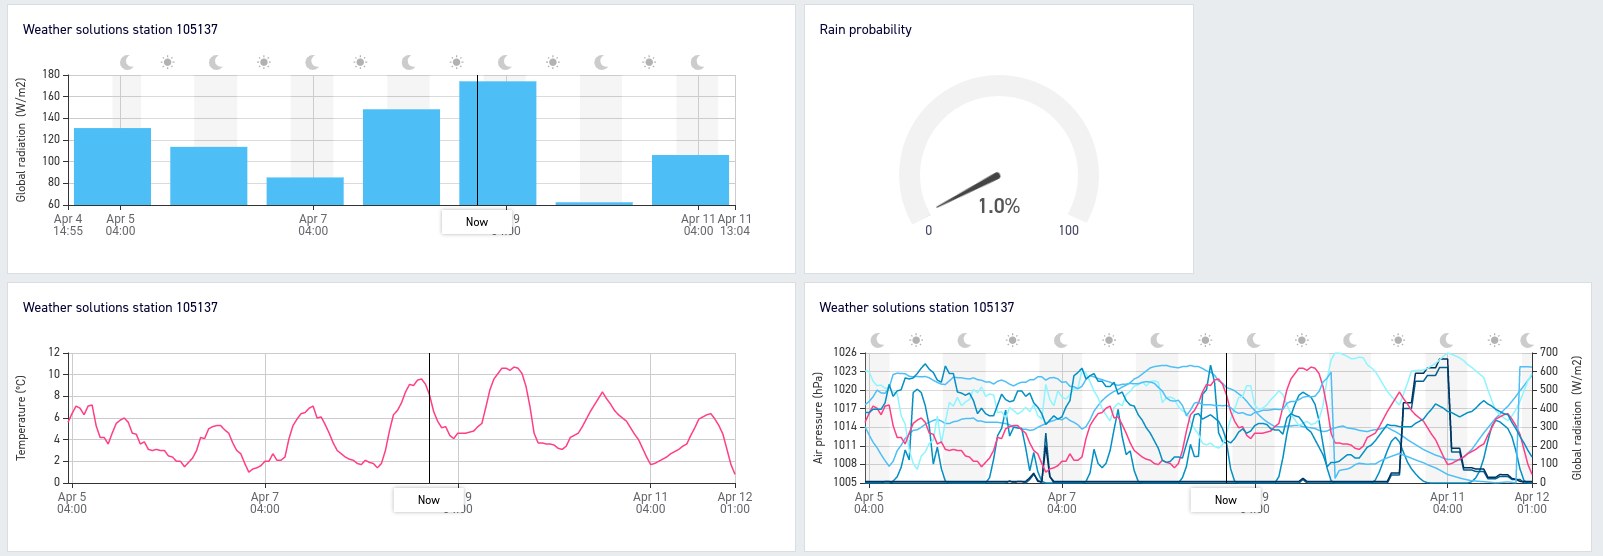
\includegraphics[width=\columnwidth]{figures/background/dashboard.png}
  \caption{Widgets in the 30MHz dashboard}
  \label{fig:bg:dashboard}
  \centering
\end{figure}

\begin{figure}[h]
  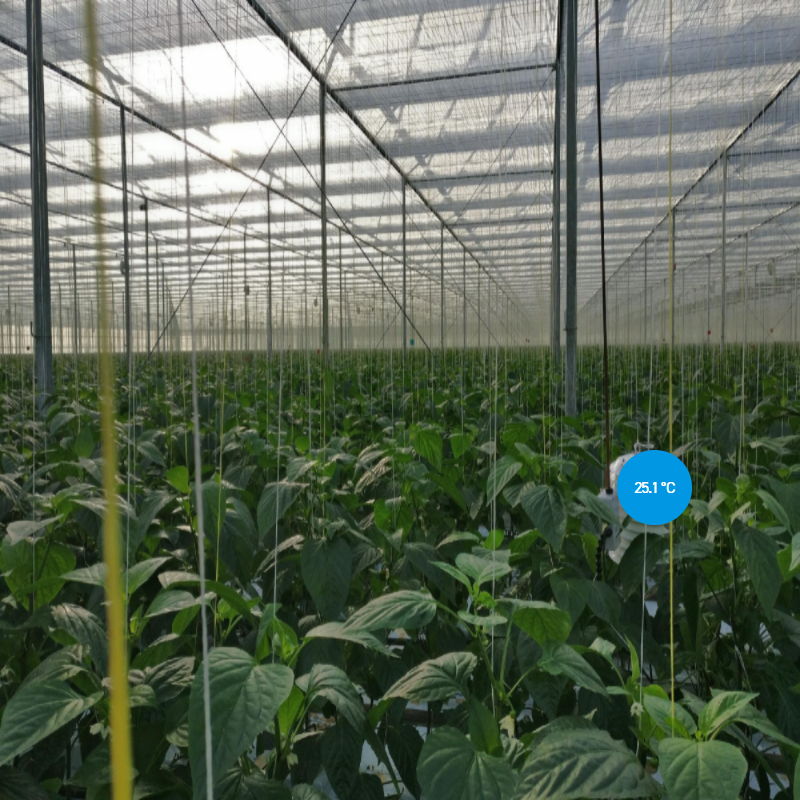
\includegraphics[width=\columnwidth]{figures/background/dashboard-img.png}
  \caption{An image widget in the 30MHz dashboard}
  \label{fig:bg:dashboard-img}
  \centering
\end{figure}

\subsection{Apps}\label{sec:bg:apps}
The data collected by 30MHz can be utilized in many ways. Companies with domain knowledge and expertise in certain areas (such as third parties) can provide customers with new insights and information that simple graphs can not. Because 30MHz itself does not have this domain knowledge and does not have the resources to create every single possible implementation of this knowledge (in the form of a widget or page in the dashboard), they decided to allow third-party developers to develop them instead. There are currently two implementations:

\begin{itemize}
  \item \emph{Widgets:} A Widget in the dashboard takes data from one or more sensors and displays it. These are made to provide information at a glance and are fairly small in screen space, as can be seen in Figure~\ref{fig:bg:dashboard}. An example would be a new way to display the amount of light a plant is getting by showing a sun icon if the plants can grow (it is daytime) and a moon icon if they are not (it is nighttime).
  \item \emph{Apps:} Full pages in the web app. These fill the entire screen (bar some 30MHz branding) and provide more rich and interactive experiences. An example would be a page where users can tune parameters (such as the number of crops, amount of watering) and see a prediction of their revenue. This prediction can be based (in part) on sensor data.
\end{itemize}

Since these apps will essentially be pages in the 30MHz dashboard and will feel like part of the platform, it is important that they follow the same design as the rest of the dashboard. A consistent design ensures that users are familiar with the apps and that visual consistency across the platform is not broken. This concept has been applied on Google's Android through Material Design~\footurl{https://material.io/} and Zendesk Garden~\footurl{https://garden.zendesk.com/} among others. Importantly, these companies all provide app developers with a set of components to help them maintain the intended design language. Such a set of components is generally referred to as a UI library.
Similarly, 30MHz wants to provide their third-party app developers with a UI library as well. In this paper, we refer to the UI library 30MHz will provide to third parties as the Cow Components UI Library (or CC UI Library). It is named after the logo of 30MHZ, a cow. There already is an internal UI library that covers the basic set of UI components (among others buttons, an input, a date picker), but since it is interwoven with other internal code, its source code can not just be provided to third-party developers. They have been written in Angular~\footurl{https://angular.io/}, meaning that any developers who wish to develop their app in a different JavaScript (JS) framework cannot do so. Looking at the most popular web frameworks in the latest Stack Overflow Developer Survey~\footurl{https://insights.stackoverflow.com/survey/2020} (2020 as of the writing of this paper), we can conclude that the chance that a developer wishes to use a different JS framework is quite large. In order to still provide developers with a CC UI library, there are two options.

\begin{itemize}
  \item Write components from scratch in a framework-agnostic format and provide them to developers. Then keep them up to date with the internal set of components by changing one as the other changes.
  \item Set up automatic conversion from the set of internal components to a framework-agnostic format.
\end{itemize}

The immediately apparent problem with the first option is that developers are maintaining two separate copies of very similar code. This causes several issues. The time spent maintaining a component is doubled. Additionally, feature differences between the Angular framework and the framework-agnostic format we choose will lead to problems. Some things that work in Angular might need workarounds in the other format and the other way around. Another issue with this option is that the components have to be written entirely from scratch. While this would be manageable for simple components such as buttons, this is unfeasible for more complex components. One such component for which this would prove difficult is the 30MHz chart component. This component is vital to the 30MHz design library, seeing as it can display the sensor data. The source code for the chart is tightly coupled with the rest of the platform, referencing about half of the source files in the dashboard through its dependencies. Rewriting all of this in another framework is wholly unfeasible and not worth the effort, leading us to explore the second option.

While the second option is not an easy one and will likely be a very complex process to set up, it will scale a lot better. Once it is set up, any new components will be automatically converted, and any changes will be propagated automatically. In the long run, this should save time. This option is the one 30MHz eventually decided on. Next, a framework-agnostic format needs to be chosen to facilitate this process.

\section{Web Components}\label{sec:bg:webcomponents}
When it comes to choosing a framework-agnostic format for a UI library, there are very few options. Looking at the literature, we find Quid~\cite{molina2019quid}, a program that allows code written in a domain-specific language (DSL) to be used to generate components in various frameworks. It currently supports the generating of Web Components~\footurl{https://developer.mozilla.org/en-US/docs/Web/Web_Components}, Stencil~\footurl{https://stenciljs.com/}, Angular and Polymer~\footurl{https://www.polymer-project.org/} components. The authors do mention it should only be used for rapid prototyping. Since it only supports a fairly small set of supported frameworks and it has the problem of requiring a DSL which the Angular code would have to be converted to, we can not use Quid as the target format.

This brings us to the other option, namely Web Components. Web Components (also known as Custom Elements) are a technology proposed in 2013~\footurl{https://www.w3.org/TR/2013/WD-custom-elements-20130514/\#about} and implemented in major browsers in 2018~\footurl{https://caniuse.com/?search=webcomponents}. It allows for the creation of custom HTML elements using JavaScript. These elements can then be used like regular HTML elements. Since every JS framework has support for native HTML elements and almost every framework has full support for Web Components~\footurl{https://custom-elements-everywhere.com/}, we can cover most JS frameworks by using Web Components as our target format.

\section{Angular Elements}\label{sec:bg:angularelements}
To perform the conversion of Angular components to Web Components, we use Angular Elements~\footurl{https://angular.io/guide/elements}. Angular Elements is a JS package that allows the conversion of Angular components to Web Components. Angular apps are typically mounted to the page by the user through a call to the \code{bootstrapModule} function. Consequently, the bootstrap component is mounted to the page. This bootstrap component is responsible for containing the rest of the application. After it is mounted, child components are mounted and rendered within its root recursively. Angular Elements works slightly differently. Components registered as Web Components through Angular Elements are instead rendered whenever an HTML element with the registered tag is added to the DOM\@. When this happens, a new root is created in place of this new HTML element. Instead of a single root in which everything is rendered (as is the case in a typical Angular app), components are all rendered in their own local root. We use Angular Elements for the conversion to Web Components in this case study since it appears to be the only package providing this task.

\begin{figure}[h]
  \caption{An example of a component that provides type hints (these hints are also referred to as intellisense)}
  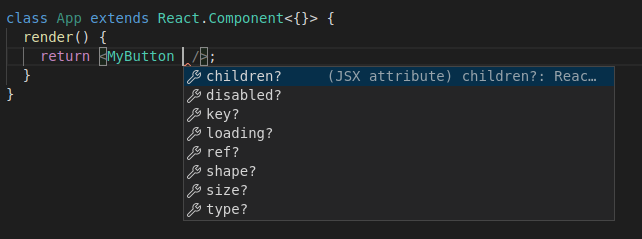
\includegraphics[width=\columnwidth]{figures/background/hinting.png}
  \label{fig:bg:hinting}
  \centering
\end{figure}

\begin{figure}[h]
  \caption{An example of a component without type hints}
  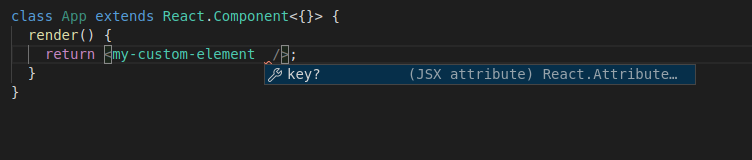
\includegraphics[width=\columnwidth]{figures/background/no-hinting.png}
  \label{fig:bg:no-hinting}
  \centering
\end{figure}

\section{Javascript frameworks}\label{sec:bg:jsframeworks}
While converting components to Web Components makes them usable in most JS frameworks, they do not provide a perfect experience. The first reason for this is them not being perfectly compatible with every JS framework. As of the writing of this paper, there are still some issues preventing them from working entirely in ReactJS~\footurl{https://reactjs.org/}, a JS framework created by Facebook in 2013. These issues mostly concern the passing of non-primitive data to the components, such as JavaScript Objects, Arrays, and Functions. The second problem is that they are not native to JS frameworks and do not integrate very well with the tooling provided by the framework. An example of type hinting provided by the framework and editor can be seen in Figure~\ref{fig:bg:hinting}. Compared to Figure~\ref{fig:bg:no-hinting}, which shows a component with no type hinting, Figure~\ref{fig:bg:hinting} provides the developer with much more information and shows them what options are available to them. Instead of searching the web for the available properties, they are provided by the element's source code and displayed by the framework tooling and editor. In order to improve the developer experience, we will provide what we will call a \emph{wrapper} for each framework. This wrapper has two functions. Firstly, it provides the tooling mentioned above. Secondly, it bridges the gap with JS frameworks that do not natively support Web Components yet. This wrapper is native to the framework, being written using the language and library the provides. This allows the framework to infer information from the wrapper's source code. Under the hood, this wrapper still uses the components in the Web Components UI library to render the components. This wrapper serves as glue code between the framework and these components. By combining the two steps of converting the original Angular components to Web Components, and the Web Components to wrappers for frameworks, we can provide developers with an experience native to their framework, even though the original source code uses Angular.

\section{UI Libraries}\label{sec:bg:ui-libraries}
As mentioned before, a set of components that adheres to one cohesive design language is generally referred to as a UI library or design library. There are two methods for implementing a design library, with one being based on doing most of the work in JavaScript and the other being based on shifting this work to CSS. The former is also referred to as a design library, with the latter being called a CSS framework. The idea of a CSS framework is to put almost all of the styles a developer will need in a single CSS file. This includes the various variations they could need. For example, a CSS library could include the \code{.padding-5} selector as well as the \code{.padding-2} selector for setting the padding of a component. Note that the number of pixels of this padding is included in the selector. This generally leads to relatively big CSS files, which may or may not be tree shaken. This is in contrast to JavaScript-based UI libraries, which generally use per-component stylesheets instead of global stylesheets. They also tend to shift numbers and sizes to JavaScript or HTML\@. For example the same padding as above could be applied through a property, i.e. \code{<my-component padding="2"/>} or \code{<my-component padding="5"/>}. This approach has the advantage of a more per-component focus, more flexibility, and options that are easier to discover. However, compared to CSS frameworks, JS-based UI libraries are significantly slower. The CSS frameworks generally only append an element to the DOM and apply some pre-computed set of classes to them, meaning they only interact with the swift JavaScript APIs that are native to the browser. JS-based UI libraries, on the other hand, generally have to run a lot more code. Since this performance difference is important when it comes to measurements, a given library being a UI library or CSS framework, is mentioned later.

\section{Related Work}\label{sec:related-work}

There are various fields in which the related work is important to us in this paper. Namely related work in the area of UI Libraries, Angular Elements (and the accompanying process of converting to Web Components), related work on Web Components themselves, and related work on the creation of wrappers around Web Components to target JS frameworks.

\subsection{UI Libraries}
We found a few studies that cover the area of UI libraries. In~\cite{ky2019ui}~\cite{annala2017documentation}~\cite{mrazcomponent}, the authors all build UI libraries. They focus mostly on the technologies used, how they work, and how they contribute to the building of the UI library. Looking at blog posts, we find numerous posts on Web Components. In these blog posts~\footurl{https://www.toptal.com/designers/ui/design-framework}~\footurl{https://dev.to/giteden/building-a-ui-component-library-for-your-startup-4cek}~\footurl{https://www.emergeinteractive.com/insights/detail/how-to-ux-ui-design-system-component-library/}~\footurl{https://codeburst.io/building-an-awesome-ui-component-library-in-2020-a85cb8bec20}~\footurl{https://itnext.io/building-a-scalable-ui-component-library-4607de91955a}, the authors provide guidance in setting up and creating a UI library. These blog posts mainly concern the basics, explaining how to get started with the process. We also find numerous examples of UI libraries. Some examples are Svelte Material UI~\footurl{https://sveltematerialui.com/} (written in Svelte), React Bootstrap~\footurl{https://react-bootstrap.github.io/} (React), Angular Material~\footurl{https://material.angular.io/} (Angular), Wired Elements~\footurl{https://wiredjs.com/} (Web Components), Onsen~\footurl{https://onsen.io/} (multi-framework), and SyncFusion~\footurl{https://www.syncfusion.com/}. For all but the SyncFusion, the source code is freely available on GitHub, allowing us to draw inspiration from it and look at how various problems were solved in different UI libraries.

\subsection{Angular Elements}
Research on the area of Angular Elements is very sparse. In our search, we only found a single paper on this subject. In~\cite{armengol2020development}, Angular Elements is used to convert form components to Web Components so that they can be rendered dynamically. On the other hand, blog posts on this area are numerous. In various blog posts~\footurl{https://netbasal.com/understanding-the-magic-behind-angular-elements-8e6804f32e9f}~\footurl{https://medium.com/kitson.mac/wrapping-an-angular-app-in-a-custom-element-web-component-angular-element-in-4-simple-steps-ded3554e9006}~\footurl{https://medium.com/@smarth55/angular-elements-use-them-everywhere-including-your-angular-app-697f8e51e08d}~\footurl{https://blog.piotrnalepa.pl/2020/02/02/how-to-convert-angular-component-into-reusable-web-component/}~\footurl{https://medium.com/swlh/angular-elements-create-a-component-library-for-angular-and-the-web-8f7986a82999}~\footurl{https://www.thirdrocktechkno.com/blog/angular-elements/}~\footurl{https://juristr.com/blog/2019/04/intro-to-angular-elements/}~\footurl{https://studiolacosanostra.github.io/2019/07/19/Build-a-reusable-Angular-library-and-web-component/}~\footurl{https://blog.bitsrc.io/using-angular-elements-why-and-how-part-1-35f7fd4f0457}~\footurl{https://www.techiediaries.com/angular/angular-9-elements-web-components/}~\footurl{https://indepth.dev/posts/1116/angular-web-components-a-complete-guide}~\footurl{https://indepth.dev/posts/1228/web-components-with-angular-elements}, the authors explain how to set up Angular Elements and how to use it to create a new component library. These blog posts mostly focus on creating new components or converting simple components through Angular Elements, not so much on converting larger and more complex components. They all use new and empty projects, contrary to two other blog posts~\footurl{https://blog.nrwl.io/upgrading-angularjs-to-angular-using-elements-f2960a98bc0e}~\footurl{https://medium.com/capital-one-tech/capital-one-is-using-angular-elements-to-upgrade-from-angularjs-to-angular-42f38ef7f5fd}. The authors use Angular Elements to convert existing AngularJS (an older version of Angular) components to the newer Angular. They do this by converting the source code of existing AngularJS components to Angular source code. By itself, this would break since the application root still runs on AngularJS and is unable to handle Angular code. By using Angular Elements to convert the Angular code into Web Components, the Web Components are able to run inside the AngularJS root. This is thanks to the low-level nature of Web Components, allowing any framework that can render HTML elements to use them. Through this iterative process, they are able to convert components one by one, converting the root component once all of its children have been converted as well.

Unfortunately, we were unable to find any related work on the conversion of complex Angular components to Web Components through Angular Elements. Related work seems to focus mostly on small get-started style projects. In the cases where they do focus on more complex projects, it seems like the only use is the conversion from AngularJS to Angular.

\subsection{Web Components}
\todo{Web Components section}

\subsection{JS Framework Wrappers}
We were unable to find any research on JS framework wrappers. This does not seem to be a problem that has been tackled very often, at least in literature. On the website \emph{custom-elements-everywhere.com}~\footurl{https://custom-elements-everywhere.com/}, the authors keep track of the current usability of Web Components in various JS frameworks. Notably, the ReactJS framework does not fully support Web Components at the time of writing for this paper. In ReactJS, non-primitive values (such as Objects, Arrays, and Functions) can not be passed to Web Components, along with some other issues. As such, it is the only framework that needs a wrapper for the UI library to function at all. Looking at how to fix this issue, we find some proposed solutions in a blog post~\footurl{https://itnext.io/handling-data-with-web-components-9e7e4a452e6e}. In this blog post, the author explores various options to tackle this problem of passing non-primitive data.
\chapter{Study Design}\label{chap:design}

\section{Research questions}
Our goal in this paper is to evaluate the effectiveness of migrating Angular components to Web Components. Based on this goal, a single research question has been devised:
\\
\\
\textbf{RQ1: How technically viable is the process of migrating Angular components to Web Components?}
\\
In answering this research question, we assess whether the migration process is possible at all, what a possible performance impact could be, and how the result relates to other component libraries in the field
\\

\section{Metric definitions}
In order to answer the above research questions, we need to define metrics. These allow us to compare the resulting Web Component library both to the UI library and to other UI libraries. This allows us to get a better understanding of the quality and performance of the created Web Component library relative to other UI libraries. We can divide the metrics used into two categories. The first is measuring the effectiveness of the resulting CC UI library. In order to do this, we compare the components in the CC UI library to the Angular components they originate from, as well as to various UI libraries. We perform this comparison using various metrics at both component granularity and at UI library granularity. A full list of these metrics, as well as a brief description, can be seen in Table~\ref{tab:design:metrics}. A detailed explanation of these metrics follows.


\begin{table}[h]
  \tiny
  \begin{tabularx}{\textwidth}{|l|l|l|X|}
    \toprule
    \textbf{ID} & \textbf{Metric}        & \textbf{Granularity}             & \textbf{Description}                                                                                                              \\ \midrule
    SC          & Structural complexity  & Component                        & The number of import statements for a component. Collected for a source file and all of its dependencies for up to two iterations \\ \hline
    CC          & Cyclomatic complexity  & Component                        & A quantitative measure of the number of linearly independent paths through a program's~\cite{1702388}                             \\ \hline
    LOC         & Lines of code          & Component                        & The number of lines of code in a given component's source file                                                                    \\ \hline
    MA          & Maintainability        & Component                        & A derivative based on complexity, lines of code and Halstead volume~\cite{halstead1977elements}                                   \\ \hline
    RT          & Render Time            & Component                        & The render time of a given component                                                                                              \\ \hline
    SI          & Size                   & UI Library                       & The file size of the bundled up library                                                                                           \\ \hline
    LT          & Load Time              & UI Library                       & Parsing and running time of the bundled up library in the browser (without download time)                                         \\ \hline
    NOC         & Number of Components   & UI Library                       & The number of components in a UI library                                                                                          \\ \hline
    FC          & First Paint            & UI Library (cow-components only) & First paint event of the browser                                                                                                  \\ \hline
    FCP         & First Contentful Paint & UI Library (cow-components only) & First paint event of the browser that includes content for the user  (text, images, etc.)                                         \\
  \end{tabularx}
  \caption{Metrics used in this study}
  \label{tab:design:metrics}
\end{table}

\subsection{Source code metrics}
The first set of metrics, namely structural complexity, cyclomatic complexity, lines of code, and maintainability, are metrics that are recommended by Martinez-Ortiz \etal{}~\cite{martinez-ortiz2016quality} as described in Section~\ref{sec:related-work:metrics}. We use these metrics to compare the quality of our Web Components to other Web Components. We follow almost all recommendations by the paper, including collecting the structural complexity up to a depth of two. Note that we do things slightly differently from the paper. We also keep track of the lines of code metric, which the authors do not. We do not use this to compare the quality of Web Components but instead we use it to get a rough overview of the complexity of various UI libraries. Note that we are also not using all metrics recommended by the authors. The metrics we are not using are the completeness (i.e.~how complete the information displayed to the user is) and consistency(i.e.~how long it takes for data to update across different replicas) metrics. We are not using completeness because it does not apply at the level at which the CC UI library operates. All of our components are 100\% complete, as well as the components of the UI libraries we compare the CC UI library to. As such, it does not make for a very interesting metric. This metric is very effective when more complex components such as entire pages are concerned, but that is not the case here. We also do not use the consistency metric. The reason for this is relatively simple, namely that we do not have any components with the ability to update across different replicas. The same goes for the UI libraries with which we compare it.

\subsection{Size}
The size metric aims to measure the theoretical impact of loading the UI library over the network. We measure this at UI library level granularity since the contributions of individual components are very hard to measure. This should serve as a good indication of the relative network loading time of UI libraries without introducing the variable of network speed. In order to differentiate between a relatively large library and a library that has many components, we also keep track of the number of components metric.

\subsection{Load Time}
The load time metric aims to provide a measure of the real impact of a UI library on the page by measuring the real-world load time. The load time we measure is the load time of the main JS bundle. This contains the code needed to register the components to the page, as well as the rendering. Note that we only measure the parsing time and running time of the JavaScript bundle. We explicitly exclude the download time from this metric since this is already captured in SI\@. A more in-depth definition of how this metric is captured is discussed in section~\ref{sec:experimental-setup:load-time}.

\subsection{First Paint \& First Contentful Paint}
The first paint metric, along with the FCP metric, are on just the cow-component UI libraries. These metrics give us an indication of the real-world load time of a page containing the CC UI library and the original components. We use these metrics to evaluate how the paint time of the UI libraries has changed after its conversion to Web Components and its later conversion to JS framework wrappers. While these metrics do not serve as a perfect way to measure the perceived load time of a page, as discussed in Section~\ref{sec:related-work:load-time}, they should serve as an excellent comparison between the various UI libraries. Since each of them contains the exact same content and is derived from the exact same source code, imperfections in these metrics are applied to all test subjects equally.

\subsection{Render Time}
Finally, the render time metric aims to capture the duration of the render cycle. We will define this render time as the time between setting the component's visibility to true and the browser being done with the rendering process. If the render time of components in the CC UI library is significantly higher than components in other UI libraries or the Angular components they originate from, the performance impact of migrating Angular components to Web Components will be too significant. If it is slightly higher, the same, or lower, we can conclude that the performance impact is minimal.

In order to obtain an objective measurement of the rendering time that is independent of user perception, we chose to measure the render time of individual components. Since the components we use in our comparisons all load in a single stage (they are either not visible or visible), there is no loading state that could cause ambiguity.

\section{Metric targets}
In order to get a sense of the state of the CC UI library, we need to compare it to other UI libraries. To do so, we have gathered a list of various UI libraries targeting the most popular JS frameworks. These most popular frameworks are React, Angular, Vue, and Svelte~\footurl{https://2020.stateofjs.com/en-US/technologies/front-end-frameworks/}. This way, we can compare the wrapper targeting a specific JS framework with UI libraries that also target that JS framework, allowing us to observe the influence of the framework itself on the various metrics. These UI libraries were gathered by searching for the terms ``Design Library'', ``UI Library'', ``javascript UI Library'', ``Svelte UI library'', ``React UI Library'', ``Vue UI Library'', ``Angular UI Library'', and ``Web Component UI Library'' on Google. We then added any UI library to the list that we came across, either by finding it as a direct result or it being mentioned in a blog post or article. A list of the UI libraries we found and the number of stars on their GitHub page can be found in Table~\ref{tab:design:ui-libraries}. While this is not a complete list of all UI libraries, we feel like it is an accurate representation of the most popular UI libraries since it contains all of the biggest UI libraries, as confirmed by the numerous blog posts listing them in order. In order to get a reasonably accurate representation of libraries using each JS framework, we selected the three UI libraries with the most GitHub stars per JS framework. The list of included UI libraries can also be seen in Table~\ref{tab:design:ui-libraries}. In addition to comparing the CC UI library against other UI libraries, we also compare it against the Angular components from which they originate. We do this by applying our metrics to the 30MHz dashboard and the relevant components within it.

Since the components included in the selected UI libraries vary greatly, we can not make a proper comparison between individual components of the UI library. For example, a button component can not be compared with a date picker component since date pickers tend to be more complex. Higher rendering times can not be attributed to the UI library running it but to the component itself. In order to be able to compare every UI library, we have selected a set of basic components that are available in every UI library. These are the Button, Input, and Switch (or Checkbox). Since every UI library contains all of these, we can compare the metrics for a single component across all UI libraries. We only apply the various metrics to these three components in each UI library. We also include a stripped-down version of the CC UI library in the set of UI libraries of which we gather metrics. This version only contains the three components mentioned above and allows for a fair comparison with other UI libraries. The reason for this is further explained in Section~\ref{sec:experimental-setup:size}.

\begin{table*}[t]
  \tiny{}
  \begin{tabularx}{\textwidth}{p{0.15\textwidth} |p{0.1\textwidth} | p{0.18\textwidth} | p{0.07\textwidth} | p{0.1\textwidth} |p{0.4\textwidth}  }
    \toprule
    \textbf{UI Library}     & \textbf{Github Stars}   & \textbf{JS Framework} & \textbf{Included} & \textbf{Version} & \textbf{Website}                                                                 \\ \midrule
    Svelte Material UI      & 1.6k                    & Svelte                & Yes               & 2.0.0            & \url{https://sveltematerialui.com/}                                              \\ \hline
    Smelte                  & 889                     & Svelte                & Yes               & 1.1.2            & \url{https://smeltejs.com/}                                                      \\ \hline
    Svelte-MUI              & 237                     & Svelte                & Yes               & 0.0.3-7          & \url{https://svelte-mui.ibbf.ru/}                                                \\ \hline
    Svelteit                & 51                      & Svelte                & No                & -                & \url{https://docs.svelteit.dev/}                                                 \\ \hline
    Material UI             & 67.1k                   & React                 & Yes               & 5.0.0-alpha.28   & \url{https://material-ui.com/}                                                   \\ \hline
    React Bootstrap         & 19.2k                   & React                 & Yes               & 1.5.2            & \url{https://react-bootstrap.github.io/}                                         \\ \hline
    React Semantic UI       & 12.2k                   & React                 & Yes               & 2.0.3            & \url{https://react.semantic-ui.com/}                                             \\ \hline
    Evergreen               & 10.6k                   & React                 & No                & -                & \url{https://evergreen.segment.com/}                                             \\ \hline
    Rebass                  & 7.2k                    & React                 & No                & -                & \url{https://rebassjs.org/}                                                      \\ \hline
    Grommet                 & 7.1k                    & React                 & No                & -                & \url{https://v2.grommet.io/}                                                     \\ \hline
    Baseweb                 & 6.2k                    & React                 & No                & -                & \url{https://baseweb.design/}                                                    \\ \hline
    Ant Design              & 5.3k                    & React                 & No                & -                & \url{https://ant.design/}                                                        \\ \hline
    Elemental UI            & 4.3k                    & React                 & No                & -                & \url{http://elemental-ui.com/home }                                              \\ \hline
    Zendesk Garden          & 858                     & React                 & No                & -                & \url{https://garden.zendesk.com/}                                                \\ \hline
    Shards React            & 649                     & React                 & No                & -                & \url{https://designrevision.com/docs/shards-react/getting-started }              \\ \hline
    Angular Material        & 21.3k                   & Angular               & Yes               & 12.0.0-next.5    & \url{https://material.angular.io/}                                               \\ \hline
    NG-Bootstrap            & 7.7k                    & Angular               & Yes               & 9.1.0            & \url{https://ng-bootstrap.github.io/\#/home }                                    \\ \hline
    NGX-Bootstrap           & 5.3k                    & Angular               & Yes               & 7.0.0-rc.0       & \url{https://valor-softw2are.com/ngx-bootstrap/\#/ }                             \\ \hline
    NG-Lightning            & 886                     & Angular               & No                & -                & \url{https://ng-lightning.github.io/ng-lightning/\#/ }                           \\ \hline
    Alyle                   & 236                     & Angular               & No                & -                & \url{https://alyle.io/}                                                          \\ \hline
    Blox Material           & 143                     & Angular               & No                & -                & \url{https://material.src.zone/}                                                 \\ \hline
    Mosaic                  & 117                     & Angular               & No                & -                & \url{https://mosaic.ptsecurity.com/button/overview }                             \\ \hline
    Element                 & 49.8k                   & Vue                   & Yes               & 1.0.2-beta.40    & \url{https://element-plus.org/\#/en-US}                                          \\ \hline
    Vuetify                 & 30.2k                   & Vue                   & Yes               & 2.4.9            & \url{https://vuetifyjs.com/en/}                                                  \\ \hline
    Quasar                  & 18.3k                   & Vue                   & Yes               & 1.15.10          & \url{https://quasar.dev/ }                                                       \\ \hline
    Ant Design Vue          & 14.1k                   & Vue                   & No                & -                & \url{https://2x.antdv.com/docs/vue/introduce }                                   \\ \hline
    Bootstrap Vue           & 13.1k                   & Vue                   & No                & -                & \url{https://bootstrap-vue.org/ }                                                \\ \hline
    Vue-material            & 9.3k                    & Vue                   & No                & -                & \url{https://vuematerial.io/ }                                                   \\ \hline
    Buefy                   & 8.6k                    & Vue                   & No                & -                & \url{https://buefy.org/ }                                                        \\ \hline
    Vuesax                  & 5k                      & Vue                   & No                & -                & \url{https://vuesax.com/ }                                                       \\ \hline
    Chakra                  & 1.1                     & Vue                   & No                & -                & \url{https://vue.chakra-ui.com/ }                                                \\ \hline
    Fish UI                 & 867                     & Vue                   & No                & -                & \url{https://myliang.github.io/fish-ui/ }                                        \\ \hline
    Wired Elements          & 8.5k                    & Web Components        & Yes               & 1.0.0            & \url{https://wiredjs.com/}                                                       \\ \hline
    Clarity Design          & 6.2k                    & Web Components        & Yes               & 5.1.0            & \url{https://clarity.design/}                                                    \\ \hline
    Fast                    & 5.6k                    & Web Components        & Yes               & 1.8.0            & \url{https://www.fast.design/}                                                   \\ \hline
    Material Web Components & 2.5k                    & Web Components        & No                & -                & \url{https://github.com/material-components/material-components-web-components } \\ \hline
    UI5                     & 887                     & Web Components        & No                & -                & \url{https://sap.github.io/ui5-webcomponents/}                                   \\ \hline
    Vaadin                  & 17                      & Web Components        & No                & -                & \url{https://vaadin.com/}                                                        \\ \hline
    Onsen                   & 8.3k                    & Multi-Framework       & Yes               & 2.11.2           & \url{https://onsen.io/}                                                          \\ \hline
    Primefaces (Angular)    & 1.3k                    & Multi-Framework       & Yes               & 11.3.2-SNAPSHOT  & \url{https://www.primefaces.org/primeng/}                                        \\ \hline
    Primefaces (React)      & 1.3k                    & Multi-Framework       & Yes               & 6.2.2-SNAPSHOT   & \url{https://www.primefaces.org/primereact/}                                     \\ \hline
    Primefaces (Vue)        & 1.1k                    & Multi-Framework       & Yes               & 3.3.6-SNAPSHOT   & \url{https://www.primefaces.org/primevue/}                                       \\ \hline
    Syncfusion              & unknown (not on github) & Multi-Framework       & No (paid)         & 1.0.0            & \url{https://www.syncfusion.com/}
  \end{tabularx}
  \caption{Collected UI libraries, the number of github stars and whether they were included in the study}
  \label{tab:design:ui-libraries}
\end{table*}

\section{Analysis of results}
In order to compare the collected measurements, we use the median value over a set of measurements. Compared to the average, the median minimizes the impact of outliers in a data set. Since the measurements we collect are likely to have outliers in them due to the nature of time-sensitive measurements, this statistical value is likely to be a better choice.
\chapter{Results}\label{chap:results}
The metrics described in Chapter\ref{chap:design} have been collected for the created CC UI library. Using these metrics, we are able to compare the CC UI library to the original Angular components, the various JS framework wrappers, and various other UI libraries. In the following sections, the various metrics are broken down, and the results are compared between the various libraries.

\section{Render Time}
The render time metric allows us to evaluate the direct performance impact on users once the page has loaded. We first compare the CC UI library to the original Angular components and the other JS framework wrappers. This allows us to evaluate the performance impact added by the process of conversion to Web Components, as well as the performance impact added by the JS framework wrappers. After this, we compare the CC UI library to the UI libraries listed in Table~\ref{tab:design:ui-libraries}, allowing us to evaluate the performance of the CC UI library relative to UI libraries as a whole.

\subsection{Cow Components}
As mentioned in Chapter~\ref{chap:experimental-setup}, we have measured three basic components in particular that every UI library contains. These are the Button, Switch, and Input. We have measured the time needed to render 1 instance, 10 instances, and 100 instances of this component. The various render times for the cow-components UI libraries with these numbers of components can be seen in figures~\ref{fig:results:render-time-cow-1},~\ref{fig:results:render-time-cow-10}, and~\ref{fig:results:render-time-cow-100} respectively. We first take a look at the single-component render times. When we compare the performance of the CC UI library with the original Angular components, we find the CC UI library's median render time to be 81\% and 100\% higher for the Input and Switch components, respectively, with the mean render time for the Button being 41\% lower. Other than the Angular wrapper's Button (which is 100\% slower), the wrappers' render times are very similar. The React and Svelte Button rendering times are 6\% and 12\% lower, respectively, with both the Input and Switch render times being between 172\% and 190\% higher. From this, we can conclude that, although there is a full Angular root running for each component, the performance impact for a single component is minimal. Now taking a look at the render times for 10 and 100 components, we start to see some big differences. The Web Components version can still keep up with the original components when it comes to rendering 10 components, being 5\% faster, 144\% slower, and 111\% slower for the Button, Input, and Switch components, respectively. When rendering 100 components instances, however, it is eclipsed by the original components. Render times are 250\%, 393\%, and 265\% slower for the Button, Input, and Switch, respectively. It seems that the impact of creating a new Angular root for each component does become significant with many components.
Additionally, the render times for the various JS frameworks start to differ quite a lot. We see a trend of the React and Svelte wrapper growing further away from the Web Components version, with the average of the component render times increasing by 339\% for the React wrapper and 597\% for the Svelte wrapper. The Angular wrapper moves away even further, with the average of its component render times increasing by 735\%. It seems that the performance impact for rendering a relatively small amount of components is minimal, while it scales up relatively quickly with a greater number of components. The fact that picking a JS framework to develop in is especially interesting, potentially costing a difference of 150ms over Web Components or 50ms over a different framework.

\begin{figure}[h]
  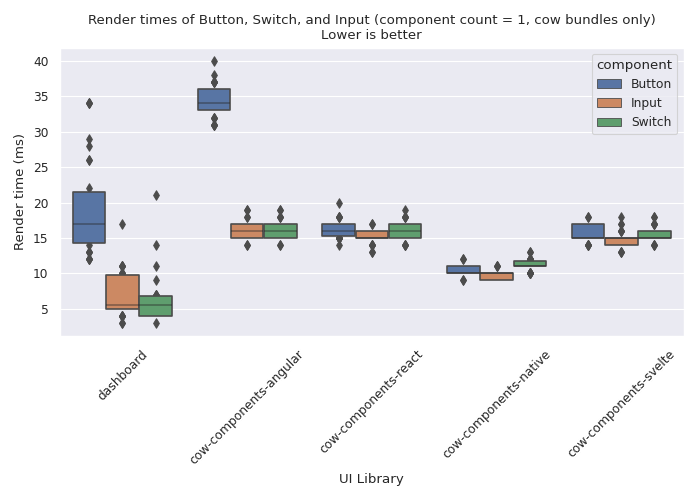
\includegraphics[width=\columnwidth]{plots/render-time-cow-1.png}
  \caption{Render times of a single Button, Switch, or Input component (CC UI only)}
  \label{fig:results:render-time-cow-1}
  \centering
\end{figure}

\begin{figure}[h]
  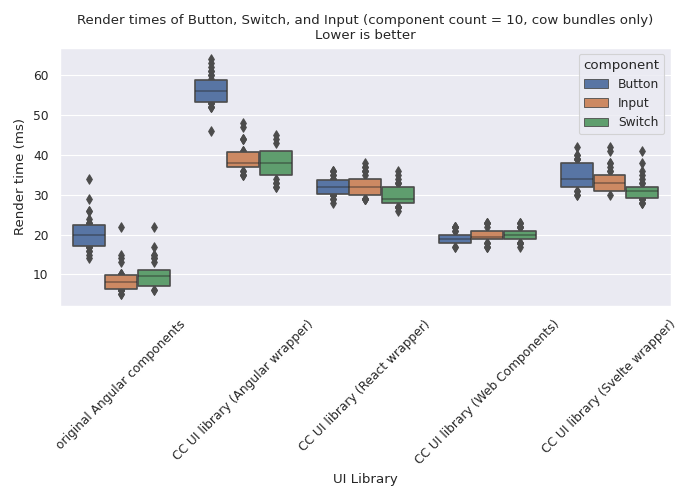
\includegraphics[width=\columnwidth]{plots/render-time-cow-10.png}
  \caption{Render times of ten Button, Switch, or Input components (CC UI only)}
  \label{fig:results:render-time-cow-10}
  \centering
\end{figure}

\begin{figure}[h]
  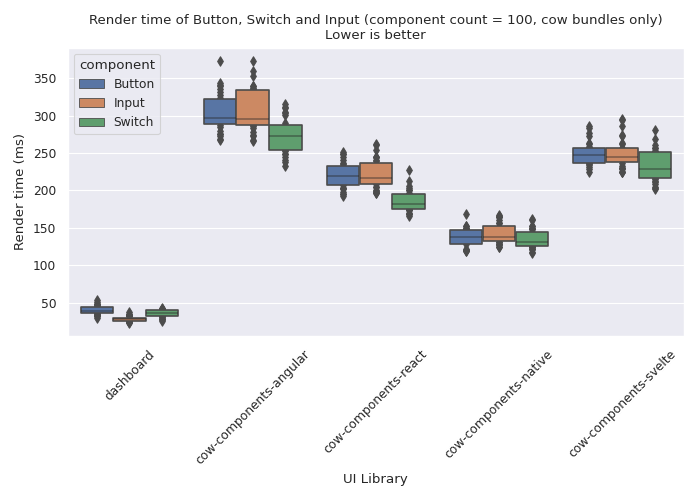
\includegraphics[width=\columnwidth]{plots/render-time-cow-100.png}
  \caption{Render times of one hundred Button, Switch, or Input components (CC UI only)}
  \label{fig:results:render-time-cow-100}
  \centering
\end{figure}

\subsection{UI Libraries}
We now compare the render times of the various UI libraries. Since the number of UI libraries we are comparing is very high (coming in at 29 total), showing them all in one figure makes for a very cluttered view. Instead, we compare a single component at a time. We have chosen to discuss the Button component in this section, however a complete overview can be found in Figures~\ref{fig:appendix:render-time-cow-1},~\ref{fig:appendix:render-time-cow-10}, and~\ref{fig:appendix:render-time-cow-100}. The render times of the Button component for the various UI libraries for 1, 10 and 100 components can be found in figures~\ref{fig:results:render-time-all-1},~\ref{fig:results:render-time-all-10}, and~\ref{fig:results:render-time-all-100} respectively.

\begin{figure}[h]
  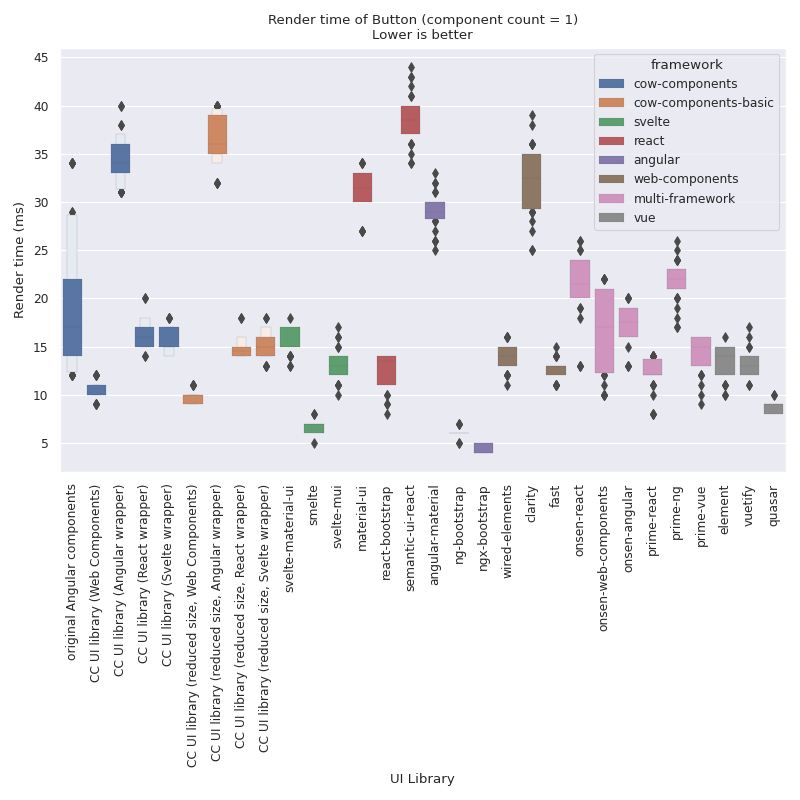
\includegraphics[width=\columnwidth]{plots/render-time-all-1-Button.png}
  \caption{Render times of a single Button. The reduced size CC UI library is the build of the library with less components, as described in Section~\ref{sec:experimental-setup:size}.}
  \label{fig:results:render-time-all-1}
  \centering
\end{figure}

\begin{figure}[h]
  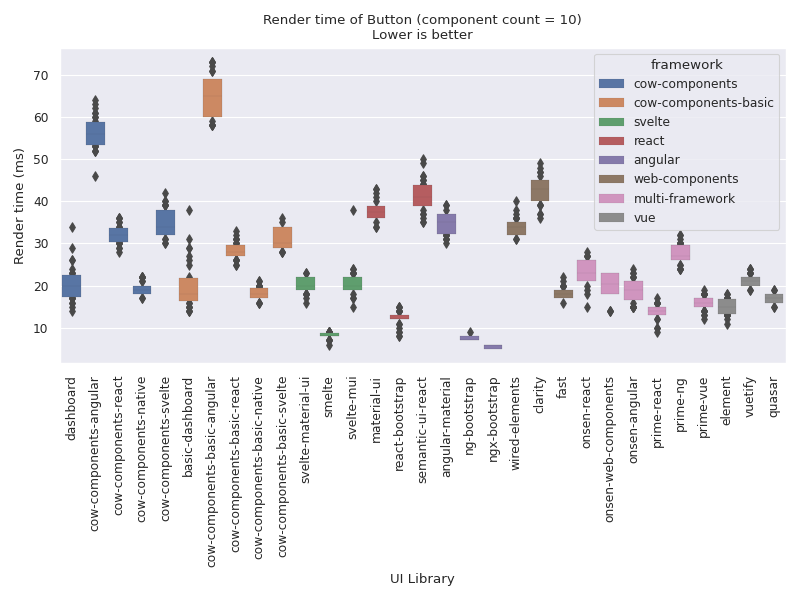
\includegraphics[width=\columnwidth]{plots/render-time-all-10-Button.png}
  \caption{Render times of 10 Buttons. The reduced size CC UI library is the build of the library with less components, as described in Section~\ref{sec:experimental-setup:size}.}
  \label{fig:results:render-time-all-10}
  \centering
\end{figure}

\begin{figure}[h]
  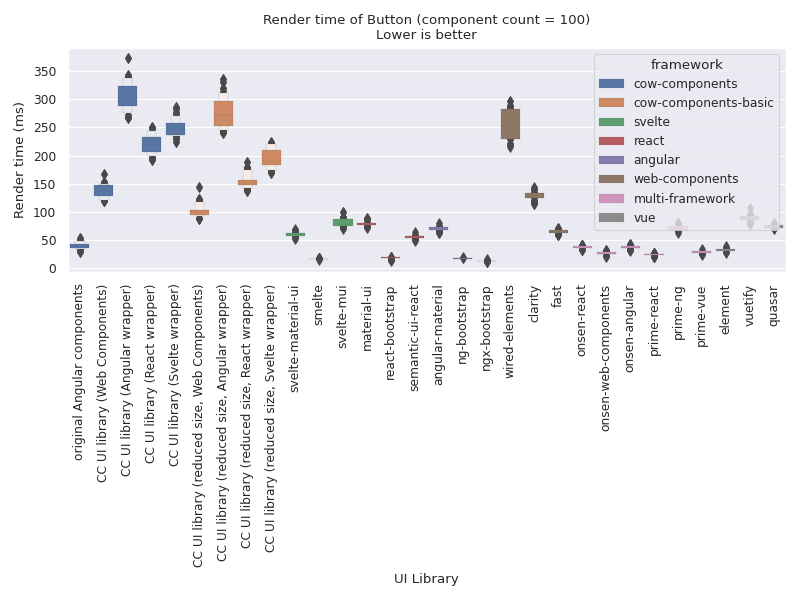
\includegraphics[width=\columnwidth]{plots/render-time-all-100-Button.png}
  \caption{Render times of 100 Buttons. The reduced size CC UI library is the build of the library with less components, as described in Section~\ref{sec:experimental-setup:size}.}
  \label{fig:results:render-time-all-100}
  \centering
\end{figure}

We, first of all, find that there are large differences in render times even within UI libraries that share the same framework. For example the render time for a button in \ver{react-bootstrap} is 57\% faster than \ver{material-ui} 64\% faster than \ver{semantic-ui-react}. In cases where this performance difference is relatively small, this has to do with the libraries themselves, but in a few cases, this has to do with the type of library. These libraries (\ver{react-bootstrap}, \ver{ng-bootstrap}, and \ver{ngx-bootstrap}) make use of a CSS framework, as laid out in section~\ref{sec:bg:ui-libraries}. As such, they are significantly faster and are essentially in a different category from the CC UI library, which is JS-based.

When we ignore these outliers, we can draw some conclusions on the average render times of the various frameworks. We first take a look at the single-component render times in Figure~\ref{fig:results:render-time-all-1}. We can see that Svelte UI libraries are generally swift, together having an average render time of 11.6ms. This falls in line with other performance benchmarks~\footurl{https://rawgit.com/krausest/js-framework-benchmark/master/webdriver-ts-results/table.html}. After this, Vue (12ms) and the UI libraries using Web Components (19,8ms) are the fastest. Interestingly, Web Components are slower than UI libraries using Svelte. Since Web Components are a native technology, one would be lead to believe that they would be faster. This might have something to do with how the authors of the UI libraries created their Web Components. It could be that their approach imposes a significant performance impact. The following frameworks when it comes to render time performance are Angular (29ms) and React (35ms). They are pretty close in performance, both being significantly slower than other frameworks. The previously mentioned performance benchmarks again support this.

We now apply our findings to the CC UI library JS framework wrappers. In our case, the Web Components version is the fastest simply because every other wrapper builds on top of this version. This means that it is impossible for another framework to be faster than it. We see this as well in the results, with the Web Components version coming in at 10ms. After that, the Svelte wrapper is the fastest, with a render time of 15ms. Interestingly, however, the React wrapper (16ms) is only slightly slower than the Svelte wrapper, while the Angular wrapper is significantly slower than both of them, coming in at 34ms. This is in contrast to what we just found, where both Angular and React were slow. It could be that the various internals of React that keep track of state and properties are slow. These are likely to be used a lot by regular React UI libraries, which need to handle their state entirely in React, while our React wrapper renders a component and passes it its properties once, making minimal use of methods exposed by React. In general, the CC UI library seems to be able to compete with the render times of other UI libraries, being faster than the vast majority of them.

\section{Load Time}
The load time metric allows us to evaluate the initial performance impact of the CC UI library. Again, we compare the various wrappers to each other as well as the original Angular components. As we elaborate on later, the Angular wrapper is significantly slower than any other UI library. For this reason, we split every figure into both a figure with and without the Angular wrapper. This should help show the scale of both this significant outlier while not reducing the scale's precision for other UI libraries.

\subsection{Cow Components}
The load time of the CC UI libraries can be seen in Figure~\ref{fig:results:load-time-cow-no-angular} (without the Angular wrapper) and Figure~\ref{fig:results:load-time-cow} (with the Angular wrapper). When we compare the load time of the CC UI library to the load time of the original 30MHz dashboard, we find that the CC UI library is significantly slower, coming in at 385ms compared to the 30MHz dashboard's 199ms. This is likely because the 30MHz dashboard has been optimized specifically for the initial load time. It loads the minimum amount of JavaScript needed to render the page. After this, other files are only loaded on an as-needed basis. The CC UI library, on the other hand, has to be contained in a single file. Splitting it up into multiple files and instructing third-party developers to have multiple JS bundles to make the CC UI library work would be a terrible developer experience. Concatenating the files into a single big bundle means all of the code has to be parsed and executed, slowing down execution by quite a lot.
Comparing the various wrappers to each other, we find the React and Svelte wrappers to have load times of 395ms and 434ms, respectively. This is only slightly slower than the CC UI library. The added load time is likely to be added by the JS frameworks themselves. Finally, we can see that the Angular wrapper is by far the slowest, with a load time of 4000ms. This is not entirely unexpected. As mentioned in Section~\ref{sec:case-study:ivy}, we had to disable AOT compilation for the Angular wrapper. This means all Angular compilation happens in the browser instead of during the compilation of the JS bundle. This is likely to be the reason why the Angular wrapper is so slow.

Taking a look at the reduced-size CC UI library, we find a loading time of 223ms for the CC UI library. This is only 12.6\% higher than the 30MHz dashboard. It appears that a significant portion of the loading was spent on these removed components. Further, the JS framework wrappers loading times are 588ms, 238m, and 277ms for the Angular, React, and Svelte wrappers, respectively. Again, the difference between the React and Svelte wrappers is minimal, with the Angular wrapper being significantly slower.

\begin{figure}[h]
  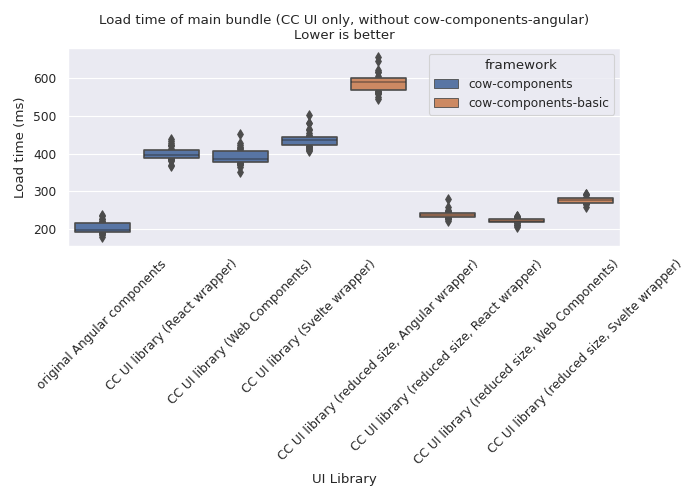
\includegraphics[width=\columnwidth]{plots/load-time-cow-no-angular.png}
  \caption{Load time of the main JS bundle (CC UI only, without Angular wrapper).}
  \label{fig:results:load-time-cow-no-angular}
  \centering
\end{figure}

\begin{figure}[h]
  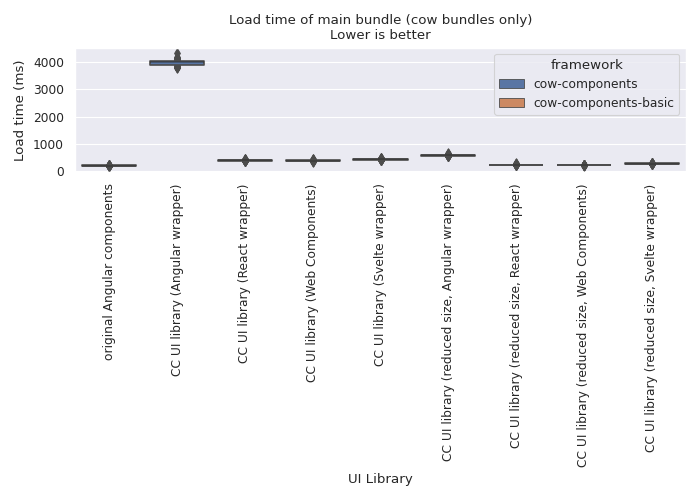
\includegraphics[width=\columnwidth]{plots/load-time-cow.png}
  \caption{Load time of the main JS bundle (CC UI only).}
  \label{fig:results:load-time-cow}
  \centering
\end{figure}

\subsection{UI Libraries}
The load times of other UI libraries can be seen in Figure~\ref{fig:results:load-time-all-no-angular} (without Angular wrapper) and Figure~\ref{fig:results:load-time-all} (with Angular wrapper). Other UI libraries largely differ in load time as well. Svelte UI libraries are by far the fastest, having an average load time of 2.64ms, followed closely by Web Components UI libraries at 11ms and React UI libraries with 22ms. After this, Vue UI libraries are the fastest, with a load time of 57ms. Finally, we have Angular, which with an average loading time of 106ms, is by far the slowest. Interestingly, we can see that the different distributions of multi-framework UI libraries follow this same pattern. For example the \ver{prime-ng} UI library is 329\% slower than the \ver{prime-react} UI library. Similarly, \ver{onsen-angular} is 167\% slower than \ver{onsen-react} and 308\% slower \ver{onsen-web-components}. This could also be one of the factors that are causing our Angular wrapper to be slower, although the lack of AOT compilation is still by far the most influential factor.

\begin{figure}[h]
  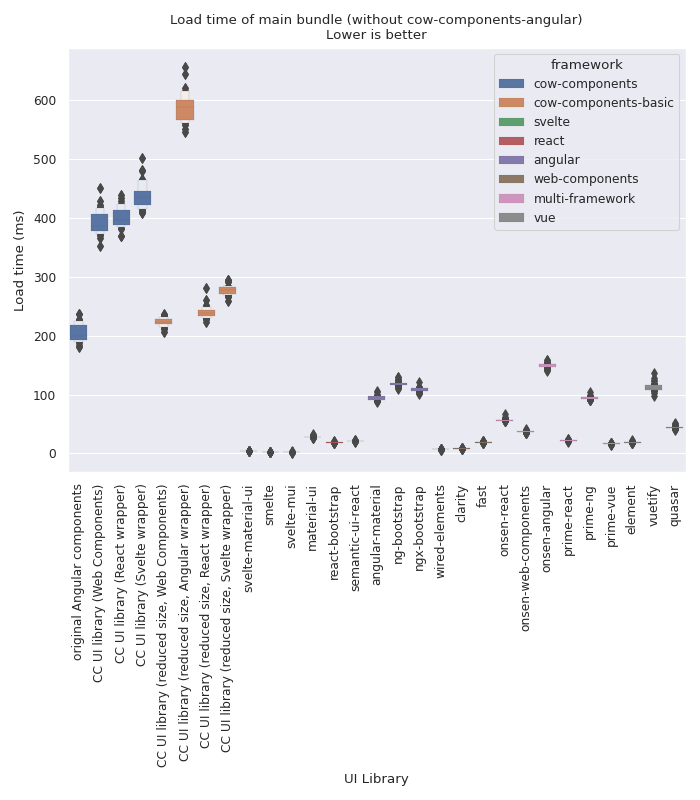
\includegraphics[width=\columnwidth]{plots/load-time-all-no-angular.png}
  \caption{Load time of the main JS bundle (without Angular wrapper).}
  \label{fig:results:load-time-all-no-angular}
  \centering
\end{figure}

\begin{figure}[h]
  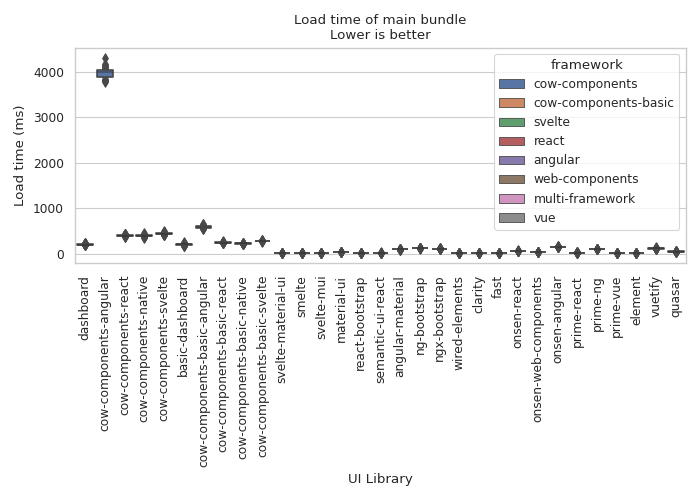
\includegraphics[width=\columnwidth]{plots/load-time-all.png}
  \caption{Load time of the main JS bundle.}
  \label{fig:results:load-time-all}
  \centering
\end{figure}

\section{Bundle Size}
Bundle size is a more abstract representation of the previous metric, allowing us to take a look at the impact of just the bundle size itself. This excludes any performance impact that can be attributed to poorly optimized code. This also allows us to look at what the performance impact of the Angular wrapper would be if there was no issue with the AOT compilation.

\begin{figure}[h]
  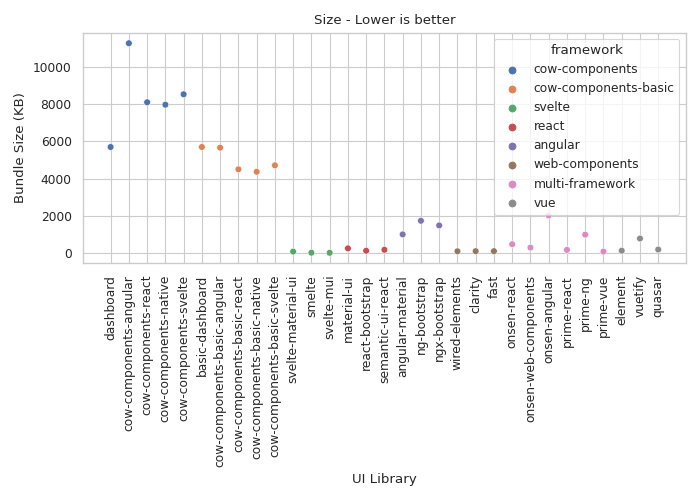
\includegraphics[width=\columnwidth]{plots/size.png}
  \caption{Size of the main JS bundle.}
  \label{fig:results:size}
  \centering
\end{figure}


The various bundle sizes can be found in Figure~\ref{fig:results:size}. We can first of all see that the bundle sizes correlate strongly with the load times. From this, we can conclude that they are an excellent representation of the load time metric. We find sizes average sizes of 57KB, 120KB, 204KB, and 385KB for Svelte, Web Component, React, and Vue UI libraries, respectively. As expected, Angular is by far the biggest, with a size of 1422KB. This same trend is also visible in our various wrappers. The Angular wrapper is by far the biggest, with a size of 11,251KB. With the strong correlation between load time and bundle size, we can conclude that a large part of the Angular wrapper's slow load time can be attributed to the large bundle size.

\section{Page Load Time}
The page load time metric should give us an idea of the real-world loading time of the CC UI library. As described in Chapter~\ref{chap:experimental-setup}, we replicated a page containing all components in the various distributions of the CC UI library. This means that all versions are rendering essentially the same page but in their own framework.

The resulting page load times can be found in Figure~\ref{fig:results:first-paint}. We have included both the \ver{First Paint} and \ver{First Contentful Paint} metrics, which are entirely the same for all the wrappers, only differing for the 30MHz dashboard. We find a first paint of 194ms and a first contentful paint of 233ms for the 30MHz dashboard. The Web Components version of the CC UI library has a first paint (and first contentful paint) of 25ms. This is 87\% faster than the 30MHz dashboard. This is likely because the dashboard also needs to run background tasks. These are tasks such as checking whether a user has logged in and fetching data. The CC UI library, on the other hand, has been stripped of this unneeded functionality. Apart from this, we can see a familiar trend of React and Svelte being slightly slower than the original, with first paint times of 618ms and 616ms, respectively. Finally, we find the Angular wrapper to have a first paint time of 2029ms.

\begin{figure}[h]
  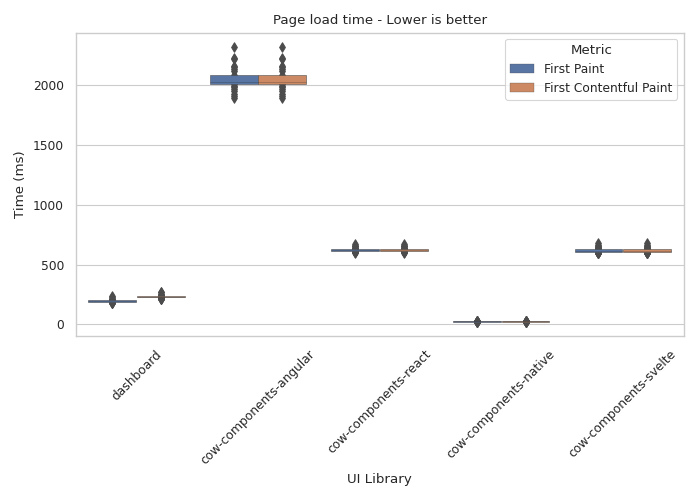
\includegraphics[width=\columnwidth]{plots/first-contentful-paint.png}
  \caption{First paint metrics for the various demo pages.}
  \label{fig:results:first-paint}
  \centering
\end{figure}

\section{Quality of Web Components}
In this section, we take a look at the quality of the Web Components in the CC UI library. Note that we essentially measure the quality of the original Angular components. This means that the conclusions drawn in this section only apply to the 30MHz codebase and will not be the same for other source codebases.

\begin{figure}[h]
  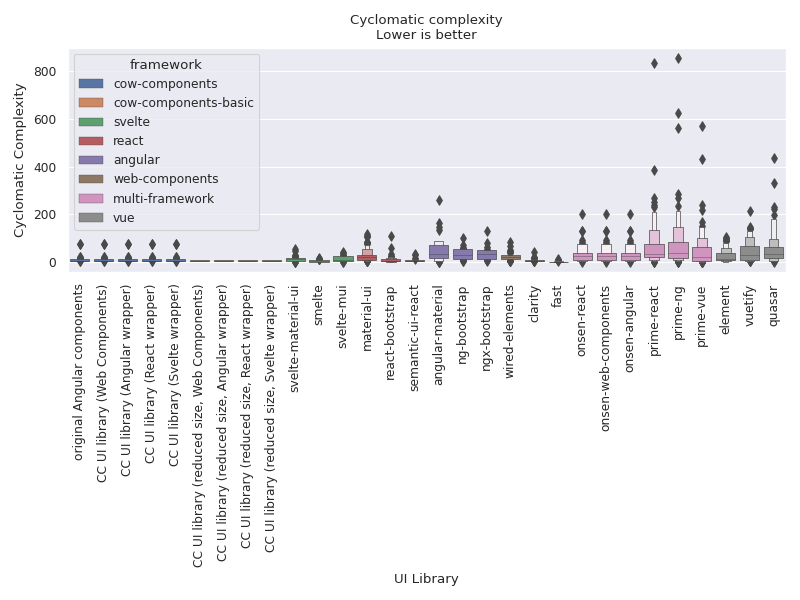
\includegraphics[width=\columnwidth]{plots/cyclomatic-complexity.png}
  \caption{Cyclomatic complexity of the various UI libraries.}
  \label{fig:results:cyclomatic-complexity}
  \centering
\end{figure}

\textbf{Cyclomatic complexity:} The cyclomatic complexities of the various UI libraries can be seen in Figure~\ref{fig:results:cyclomatic-complexity}. The cyclomatic complexity of the CC UI library is has a median value of 2 and a mean value of 10.4. The average cyclomatic complexity of the medians of all UI libraries is 17.5. Multi-framework UI libraries, in particular, have a very high cyclomatic complexity. The median cyclomatic complexity for all \ver{onsen}-based UI libraries is 22, while the cyclomatic complexities for \ver{prime-react}, \ver{prime-ng}, and \ver{prime-vue} are 31.5, 36, and 18 respectively. This makes sense since these libraries often try to share the source code between the various frameworks as much as possible, leading to many imports.

\begin{figure}[h]
  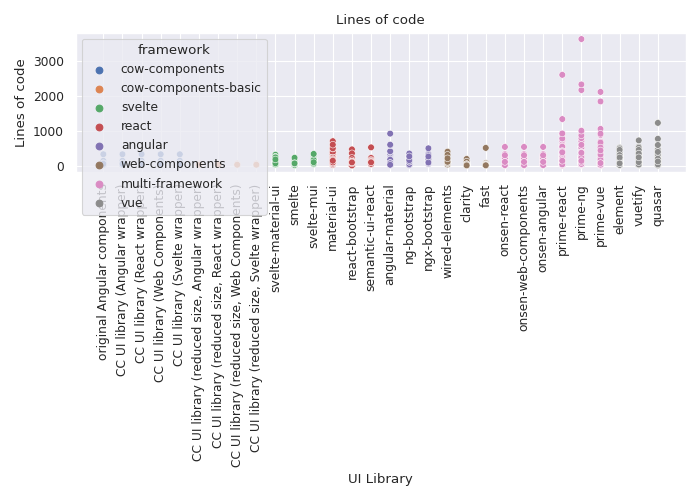
\includegraphics[width=\columnwidth]{plots/lines-of-code.png}
  \caption{Lines of code of the various UI libraries.}
  \label{fig:results:lines-of-code}
  \centering
\end{figure}

\textbf{Lines of code:} The amounts of lines of code can be seen in figure~\ref{fig:results:lines-of-code}. Again we see the same trend of the CC UI library being relatively low in complexity (and as such lines of code), with the median lines of code being 26. The average of the medians of all UI libraries is 108.75.

\begin{figure}[h]
  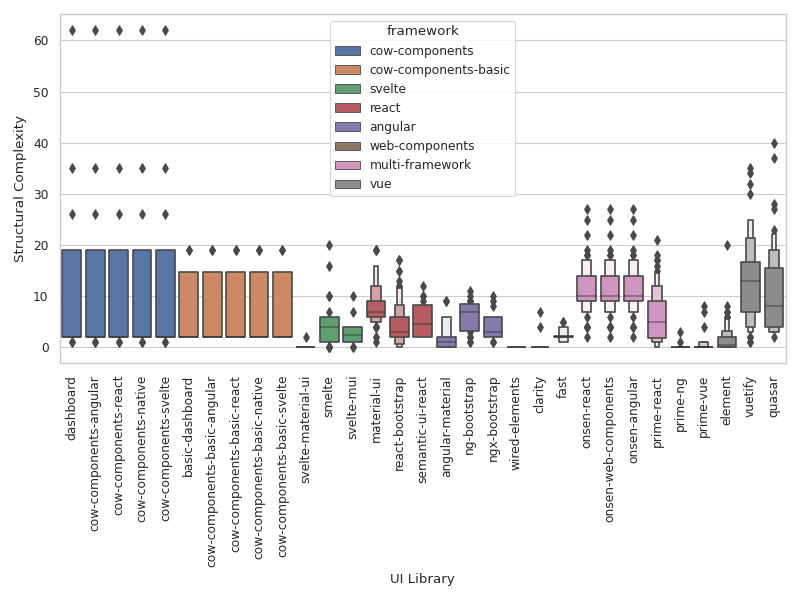
\includegraphics[width=\columnwidth]{plots/structural-complexity.png}
  \caption{Structural complexity of the various UI libraries.}
  \label{fig:results:structural-complexity}
  \centering
\end{figure}

\textbf{Structural complexity:} The structural complexities can be seen in figure~\ref{fig:results:structural-complexity}. This time there is a large variation in the structural complexity of CC UI library components, with the median being 2 and the average being 12.6. This outlier is likely to be the Chart component, which is by far the biggest component. The average of the other UI libraries' median structural complexity is 4.2. This suggests that the median structural complexity of the CC UI library is relatively low, which is good.

\begin{figure}[h]
  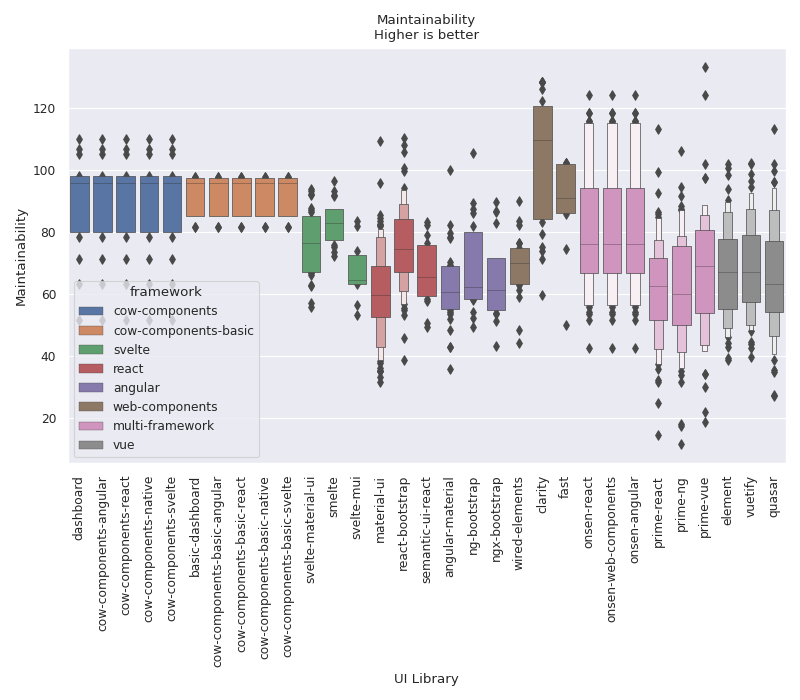
\includegraphics[width=\columnwidth]{plots/maintainability.png}
  \caption{Maintainability of the various UI libraries.}
  \label{fig:results:maintainabilty}
  \centering
\end{figure}

\textbf{Maintainability:} The maintainabilities can be seen in figure~\ref{fig:results:maintainabilty}. The median maintainability of the CC UI library is 96, with the average median maintainability of the UI libraries being 71. Higher maintainability is better, meaning the CC UI library scores quite well in this metric. All together, we can conclude that the quality of the CC UI library components (and as such, the Angular components they are based on) is quite high.

\section{Time spent on the project}\label{sec:results:time-spent}
While the technical results of this project are important, we also decided to take a look at the business side of this project. An important factor here would be the amount of effort required to complete this project. In total, this project took five months of fulltime-equivalent (FTE) to complete. An estimation would be that about one month was spent on Web Component related issues, three months on Angular related issues and one month on creating JS framework wrappers, and one month on other tasks such as creating a build pipeline and package distributions. Note that the time taken is entirely separate from the number of components in the resulting UI library, meaning an added component would not increase the time taken at all. Depending on the time required to build the UI library from scratch combined with the time taken to maintain the UI library and adding new components, this project could very well be worth it.
\chapter{Threats to Validity}\label{chap:threats-to-validity}

In this chapter, we will be covering threats to the validity of this study. Firstly we will discuss the internal validity, after which we will discuss the external validity of the study.

\section{Internal Validity}
Possible internal threats to validity would be the measurement of our metrics being influenced by external factors. As described in Section~\ref{sec:experimental-setup:load-time} we explicitly remove the factor of network speed from our benchmarks. This leaves only the factor of available system resources as a possible variable. In order to eliminate this factor, we took several steps. We first ensured a clean testing environment by shutting down all unneeded background processes on the test machine. This should vastly reduce the amount of fluctuation in available system resources. Secondly, we ensured that only a single test is running at a time. This means every test has the entire computer to itself (in practice, likely a single core) and does not compete with other tests for system resources. Lastly, we apply all the steps described in Section~\ref{sec:experimental-setup:time-sensitive-metrics} which includes randomizing the order in which the tests are run and increasing the number of tests to \numMeasures{} measurements per test. This should ensure that any possible fluctuations are smoothed out and shared across all tests.

\section{External Validity}
A large number of problems in this case study faced applied to Web Components in general, as shown in Section~\ref{sec:web-component-issues}. Still, a significant share of the problems is related to Angular, more specifically Angular 10. Likewise, a significant part of them is specific to the 30MHz codebase. Given a different codebase or a different Angular version, different problems might be faced in the process of converting Angular components to Web Components. While the issues might differ from framework to framework or even from Angular version to Angular version, the results should be generalizable to other frameworks and Angular versions. Bugs we encountered are likely to be fixed, and performance is likely to only improve in future Angular versions, as has been the case with the Angular Ivy compiler~\footurl{https://angular.io/guide/ivy}. Additionally, a significant amount of the faced problems apply to Web Components in general, as shown in Section~\ref{sec:web-component-issues}. For this reason, we believe that the feasibility of the applied process will at worst stay the same and at best improve for other Angular versions or JS frameworks.
Further, while the specific UI library we created is dependent mainly on the 30MHz codebase and its specific architecture and contents, we make sure to compare the created CC UI libraries with the original 30MHz codebase itself, ensuring all results are relative to the original. This should ensure we answer the research question for a generalized case. If we were to compare the CC UI library solely to other UI libraries, the answer to the research question would only apply to the case of 30MHz.
\chapter{Discussion}\label{chap:discussion}

The results described in Chapter~\ref{chap:results} show that the creation of a UI library from an existing codebase is very well possible in an Angular application. Render times are only slightly higher, remaining competitive with various other UI libraries. One negative aspect seems to be that the render times increase quite quickly with a higher number of components. Further, load times are not significantly higher in all cases except the Angular wrapper. This all should result in a good user experience across the board, being slightly slower than the original components but providing access to them in most popular JS frameworks. We can say that the answer to SRQ1 is that it is definitely technically feasible to convert Angular components to Web Components.

While the technical results of this project are important, we also evaluated the business side of this project through SRQ2. We find the time spent to be five months of FTE\@. We also took a look at the degree in which this project interferes with the original codebase and its developers' workflows. In questioning the three front-end developers at 30MHz, we found that on average they rated the impact of changes to the main codebase as a 2.6 on a scale from 0 (no impact at all) to 10 (significant impact). For a process that interlocks with the main codebase so heavily, this is a very low number, leading us to believe that the impact was small. Additionally, there are some new factors that developers have to keep in mind while developing new components. An example of this is the need for better documentation for components in order to ensure the automatically generated documentation is correct. Another example would be the need to add a new UI component to the array containing all components that are to be included in the UI library. On average the developers rated the impact of these changes to be a 2, signaling that the every day impact is not very large. Lastly, we asked developers how often their workflow was blocked by the existence of this project. All of them indicate they have not been blocked once, meaning this project was executed completely in parallel and without blocking other developers' workflow. These results suggest that the answer to SRQ2 is that the business viability of the conversion of Angular components to a UI library is quite high as well, leading to minimal impact on current developers and their workflow, while requiring relatively little time. Especially in a situation where there are a large number of UI components, the time spent on this project is significantly smaller than the time spent recreating them.

All in all we can conclude that the answer to RQ1 is that the process of converting Angular components to a Web Component UI library is quite feasible. We hope this case study convinces businesses who are considering this process to take the steps we have taken over the creation of an entirely new UI library. In addition to being used in the manner we described, that is the creation of a UI library for 3rd parties, this process could also be applied to components that are internal to a business. With the ever increasing amount of platforms with which users are able to interact (desktops, phones, tablets, televisions, smart fridges), the number of platforms for which businesses need to develop an application also increases. Since most of these platforms require different software stacks, Web Components could provide a basis off of which to generate components for other platforms. For example the main large web app can be built in Angular, with another small internal web app being built in React (using the React wrapper), another internal web app built in Vue, and the mobile apps built using React Native~\footurl{https://reactnative.dev/} or Apache Cordova~\footurl{https://cordova.apache.org/}.

What the results of these study do not tell us is the viability of converting components from any other JS framework to Web Components. In this case study we specifically targeted Angular, which provides the simple Angular Elements tool~\footurl{https://angular.io/guide/elements}. Other JS frameworks might not have such tools available, which might make this process less straightforward. However, we believe that the process of converting components from any other popular JS framework to Web Components may very well be significantly easier than from Angular components. A large number of the issues we faced were Angular related, as described in Section~\ref{sec:case-study:ng-deep}. Those issues were also by far the hardest to solve. Most of these issues would not appear when using other JS frameworks.

As mentioned, this case study only allows us to draw conclusions of the viability of converting \textbf{Angular} components to Web Components. As such, we think a good starting point for further research is research into this same process for other JS frameworks. If this process is proven to be viable for other JS frameworks as well, businesses would be able to convert their components to Web Components regardless of their original JS framework, allowing for this process to be far more widely used.
\chapter{Conclusion}\label{chap:conclusion}

In this case study, the feasibility of converting a set of Angular components to Web Components was evaluated. Chapter~\ref{chap:case-study} describes the various issues we faced during this project, eventually showing that it is possible to convert a set of Angular components to Web Components. In Chapter~\ref{chap:results} we evaluate the end resulting Web Components, comparing them to both the original Angular components they were created from and various other UI libraries. We find that the newly created Web Components are only slightly slower in rendering and take only about twice as much time to load. The resulting components hold up very well compared to other UI libraries, initially being faster than quite a few of them but becoming relatively slower as the number of rendered components increases. This means that although the Web Components library was converted from Angular components, it can compete quite well with other UI libraries that were written from scratch. This confirms the technical feasibility of converting Angular components to Web Components.

Further, when looking at the business side in Section~\ref{sec:results:time-spent} and Chapter~\ref{chap:discussion}, we find that the impact on the existing codebase and other developers is minimal. We also find the time spent on this conversion to be definitely worth it depending on the time required to build the UI library from scratch combined with the time taken to maintain the UI library and adding new components. This indicates that this conversion is a worthwhile investment, leading to freedom from maintaining two sets of components and the ability to easily add a new component to the Web Components library without issues. It should be noted that these results are not based on sufficient data to draw definitive conclusions. Instead, we indicate that these were our results and leave definitive proof for future work.

One shortcoming of this thesis is that we were only able to evaluate the effectiveness of converting \textbf{Angular} components to Web Components. Not the conversion of components from any JS framework to Web Components. We theorize that this process should be just as feasible, with other frameworks likely taking significantly less time to convert than Angular. As such, we believe further research into the conversion of components from other JS frameworks to Web Components would be very beneficial, eventually leading to a situation where we can conclude that components from all JS frameworks can be converted to Web Components, eventually making them re-usable across all JS frameworks.

\bibliographystyle{IEEEtran}
\bibliography{bib/references}

\end{document}






